\documentclass[../talk.tex]{subfiles}
\begin{document}

\begin{frame}{Unreliable communication}
    \begin{overlayarea}{\slidewidth}{\slideheight}
        Program sending messages over a \alert{lossy network connection}
        \begin{center}
            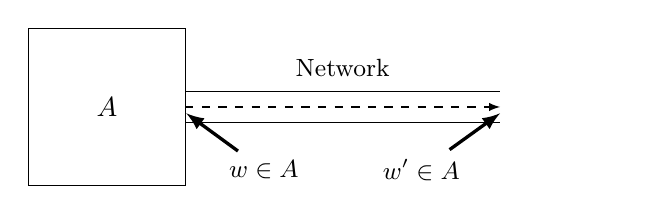
\begin{tikzpicture}
                \node [text=white] at (7,0) {dummy};
                \node (P) at (0,0) [minimum width=2cm,minimum height=2cm, anchor=west,draw] {$A$};
                    \path [->,>=latex]
                        (2,0.2) edge [-] (6,0.2)
                        (2,0) edge [dashed] (6,0)
                        (2,-0.2) edge [-] (6,-0.2)
                    ;

                    \node at (4,0.5) [font=\small] {Network};

                    \node (LP) at (3,-0.8) [font=\small] {$w \in \lang{A}$};

                    \node (LPdc) at (5,-0.8) [font=\small] {\alert{$w' \in \dc{\lang{A}}$}};

                    \path [very thick, ->,>=latex]
                        (LP) edge ([shift={(0,-0.08)}] P.east)
                        (LPdc) edge (6,-0.08)
                    ;
            \end{tikzpicture}
        \end{center}

        \begin{itemize}
            \item[] We are typically given a description of $A$
            \item[] Specification talks about $\dc{\lang{A}}$, the visible behavior of $A$
            \item[] Unreliable communication forms an environment that has to be taken into account
        \end{itemize}

    \end{overlayarea}
\end{frame}

\end{document}
